
\subsection{Equipe de projet}

\noindent
L'équipe se compose de quatre étudiants en première année :

\begin{itemize}
    \item Cheneviere Thibault
    \item Guillot Thom
    \item Hashani Elion
    \item Yebouet Antoine
\end{itemize}

\vskip 0.25cm
\noindent
Notre groupe se réunissait généralement les mardis à 15h30 dans l'école et discutait de l'avancement du projet, de nouvelles idées la concernant ainsi que de la répartition du travail à réaliser. Durant tout le projet, l'équipe communiquait à travers le réseau social Instagram.

\vskip 0.25cm
\noindent
Toute la partie Gestion de Projet a été réalisé sur le drive Google crée par le groupe. Toute la programmation a été réalisé et partagé sur le Git fourni par l'école. La rédaction du rapport a, quant à elle, été faite sur Leaf.

\subsection{Analyse du projet}
    \subsubsection{Définition des objectifs}
    Chaque work package a été attribué à chaque membre du groupe à l'aide de la méthode SMART :
    
    \begin{table}[!ht]
    \begin{tabularx}{\textwidth}{|c|l|X|}
        \hline
          & Critère     & Indicateur  \\
        \hline
        S & Spécifique  & L'objectif est défini clairement. \\
        \hline
        M & Mesurable   & L'objectif est mesurable, par des indicateurs chiffrés ou livrables. \\
        \hline
        A & Atteignable & L'objectif doit être motivant sans être décourageant et doit apporter un plus par rapport au lancement du projet. \\
        \hline
        R & Réaliste    & L'objectif doit être réaliste au regard des compétences et de l'investissement de l'équipe du projet. \\
        \hline
        T & Temporellement défini
                        & L'objectif doit être inscrit dans le temps, avec une date de fin et des jalons. \\
        \hline
    \end{tabularx}
    \label{SMART}
    \end{table}

\subsubsection{Analyse et gestion des risques}

\noindent
Une matrice SWOT (c.f. Annexe) a été réalisé pour évaluer les risques ainsi que les atouts du projet.\\
Des jalonnemens réguliers ont été effectués pour éviter l'effet tunnel dans notre projet (c.f. Annexe).

\vskip 0.5cm

\subsection{Organisation du projet}

\noindent
Le projet s'est déroulé de début novembre 2021 à début janvier 2022.\\
Nous avons réparti le travail en plusieurs étapes pour faciliter l'organisation et la réalisation de ce projet. (c.f. Annexe)
Ces étapes ont été attribués aux membres du groupe dans l'optique d'un avancement optimal du projet avec la méthode SMART.\\
La matrice RACI résume cela avec les différents lots de travail attribués.(c.f. Annexe)\\
Pour pouvoir évaluer dans le temps l'avancement du projet, un Gantt a été réalisé (voir figure \ref{fig:gantt})

    \begin{figure}[!ht]
        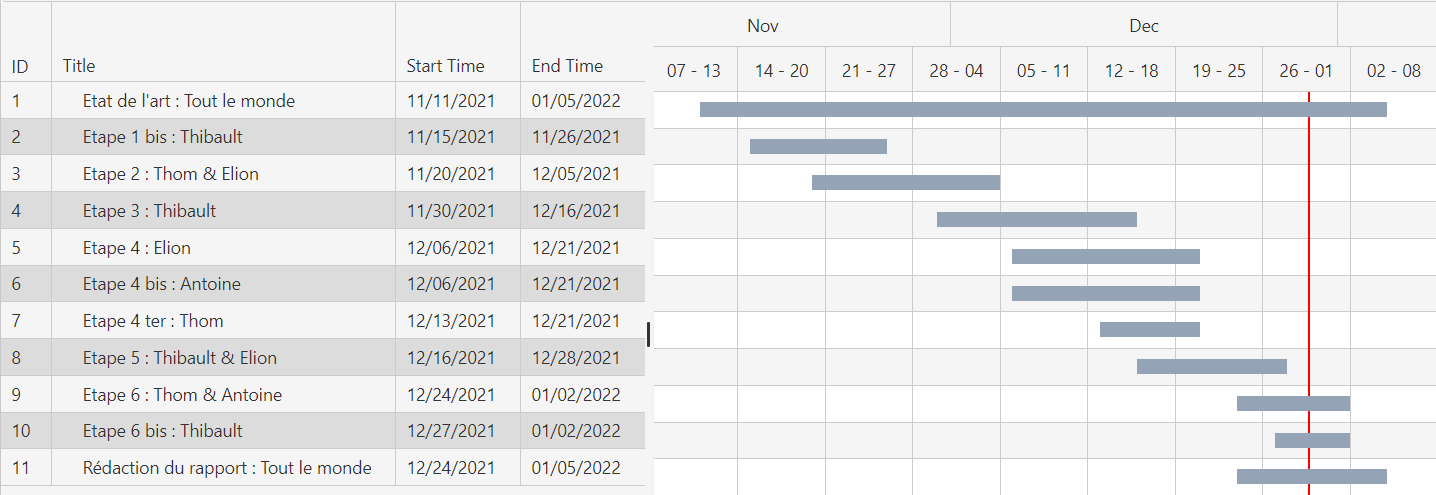
\includegraphics[scale = 0.575] {Gantt.png}
        \caption{Diagramme de Gantt (dernière version : 29/12/2021)}
        \label{fig:gantt}
    \end{figure}

\newpage
\subsection{Outils de Travail}
\noindent
Nous avons utilisé le répertoire Git fourni par l'école durant tout le projet, chaque membre du groupe avait sa propre branche dans laquelle chacun mettait son travail réalisé. Thibault gérait la branche master, avec la fusion des branches.

\subsection{Comptes-rendu des réunions}
    
    \subsubsection{9 novembre 2021}
    \vskip 0.75cm

\begin{center}
\begin{tabular}[]{|l|l|}
     \hline 
     Présent & Absent\\
     \hline
     Cheneviere Thibault &\\ Guillot Thom & \\
     Hashani Elion &\\ Yebouet Antoine &\\
     \hline
\end{tabular}
\end{center}

\vskip 0,75cm

\noindent
\textbf{Ordre du jour}

\begin{enumerate}
    \item Proposer des idées pour l'application 
\end{enumerate}

\vskip 0.75cm

\noindent
\textbf{Idées}

\noindent
\textit{Idées proposées par l'ensemble de l'équipe projet : }
    
    \begin{itemize}
        \item Trouver un moyen d’attirer les gens à voter (aller chercher les gens chez eux pour les faires voter)
        \item Sondage, 1 vote par compte (système de vérification des comptes avec unicité de la personne, par exemple système de vérification de carte d’identité). Espace avec échange d’idées (commentaire, …)
        \item Espace avec les news de la ville (politique, divers, sport, …)
        \item Compte avec des accès spécifiques (Maire, conseil municipal, admin, citoyen, …)
        \item Système de notification avec des mails, messages ou autre
        \item Système de lien avec les flux sociaux des politiciens
        \item Résumé de tous les programmes des différents partis/candidats.
        \item Faire une interface attrayante, interactive et qui attire les personnes à venir lire les informations.
        \item Faire un camembert des capacités sur 5 sujets et les personnes peuvent donner leur avis sur chaque candidat après avoir lu leur programme.
        \item Faire une interface avec un hémicycle sur lequel on peut directement cliquer pour avoir accès aux informations des candidats suivant leurs orientations politiques.
    
    \end{itemize}
 
\vskip 1cm
\noindent
\textit{TO DO LIST}
\vskip 0.25cm

\begin{itemize}
    \item Chercher des exemples et des applications de Civic Tech.
    \itemÉtablir ensuite un ensemble de critères que l’on veut avoir sur notre application.
\end{itemize}


    
    \newpage
    \subsubsection{19 novembre 2021}
    \vskip 0.75cm

\begin{center}
\begin{tabular}[]{|l|l|}
     \hline 
     Présent & Absent\\
     \hline
     Cheneviere Thibault & Guillot Thom\\ 
     Hashani Elion &\\ Yebouet Antoine &\\
     \hline
\end{tabular}
\end{center}


\vskip 0,75cm

\noindent
\textbf{Ordre du jour}

\begin{enumerate}
    \item Objectif
    \item Avancement du projet
\end{enumerate}

\vskip 0.5cm

\noindent
\textbf{Objectif}\\
\noindent
La séance d'aujourd'hui a pour but de déterminer les fonctionnalités du projet que l'on souhaite implémenter et obtenir une validation de la part des responsables du module. \\ 

\noindent
\textit{Fonctions principales}
\begin{itemize}
    \item Page de News de la ville (en page d'accueil) avec les news des clubs de la ville (sportif, artistique, culturel, …), nouvelle décision des élus (projets qui ont été acceptés).
    \item Système d’aide à la prise de décision : avant de voter un projet, permettre au citoyen de choisir le budget alloué à ce projet, impliquer les citoyens sur les plans urbains de la ville à travers des sondages (les mineurs ne pourront pas voter et il y a un vote unique par personne) et des discussions. 
    \item Système lors d'élection : présenter les programmes des différents candidats à travers un hémicycle (représentation graphique) qui répertorie tous les candidats. Les candidats écriront directement leur programme pour éviter les informations biaisées.
    \item Système d’entraide entre les riverains : faire une plateforme pour poster ses annonces pour demander de l’aide ou proposer son aide (par exemple aide pour faire du bricolage, de la mécanique, aide sur un problème avec du matériel informatique, …)
    \item Système de création de projet par les citoyens : système de budget participatif (possibilité de financer des projets de riverains) et possibilité de promouvoir un projet avec des pétitions pour les faire connaître et financer par les élues.
    \item Système de signalisation des problèmes : chaque citoyen peut signaler des incivilités ou des problèmes liés à la gestion de la ville (problème de circulation sur certains axes, problème de ramassage des poubelles dans certains quartiers, …)

\end{itemize}

\vskip 0.5cm

\noindent
\textbf{Avancement du projet}

\vskip 0.25cm
\noindent
\textit{Etape 1 bis :} \\
Thibault a commencé l'implémentation du login/authentification des candidats.
\\Elion a débuté la rédaction de la charte de projet, accompagné de la gestion du document.

\vskip 0.25cm

\noindent
\textit{Etat de l'art :}
\\Nous avons trouvé plusieurs exemples de la Civic Tech et ses exemples d'implémentations 

\vskip 1cm
\noindent
\textit{TO DO LIST}
\vskip 0.25cm

\begin{itemize}
\item Pour tous :
\begin{itemize}
    \item Attendre la réponse des responsables du modules pour démarrer l'implémentation
    \item Continuer la recherche sur la Civic Tech
    \item Réaliser la matrice SWOT
\end{itemize}
\item Pour Elion :
\begin{itemize}
    \item Terminer la charte et la gestion du document
\end{itemize}
\item Pour Thibault :
\begin{itemize}
    \item Terminer le système de login
\end{itemize}
\end{itemize}
    
    \newpage
    \subsubsection{24 novembre 2021}
    \vskip 0.75cm

\begin{center}
\begin{tabular}[]{|l|l|}
     \hline 
     Présent & Absent\\
     \hline
     Cheneviere Thibault & Yebouet Antoine\\ 
     Guillot Thom &\\ Hashani Elion &\\
     \hline
\end{tabular}
\end{center}


\vskip 0,75cm

\noindent
\textbf{Ordre du jour}

\begin{enumerate}
    \item Objectif
    \item Avancement du projet
    \item Description de l'application
\end{enumerate}

\vskip 0.25cm

\noindent
\textbf{Objectif}\\
\noindent
La séance d'aujourd'hui a pour but de clarifier la description de l’application avec les retours fait sur la première proposition. \\ 

\noindent
\textit{Objectif de l'application :}\\
L’objectif de l’application est de faciliter le vote en donnant un accès facile au programme de chaque candidat et en proposant une première analyse du programme qui pourra être affinée par les citoyens les plus investis. Ensuite la localisation des différents bureaux de vote facilite la démarche de vote pour les personnes les plus récalcitrantes.

\vskip 0.25cm

\noindent
\textbf{Avancement du projet}\\
\noindent
\textit{Etape 1 bis :} \\
Thibault a terminé l'implémentation du login/authentification des candidats.
\\Elion a fini la rédaction de la charte de projet et ainsi que celle de la gestion du document et ajoute les étapes du projet au fur et à mesure. Matrice SWOT réalisé.

\vskip 0.25cm

\noindent
\textit{Etape 2 :}\\
Thom a commencé à réaliser la page d'accueil du site

\vskip 0.25cm

\noindent
\textbf{Description de l'application}
\begin{itemize}
    \item Chaque candidat aura des identifiants pour pouvoir se connecter et entrer son programme en ligne.
    \item Ensuite après le référencement d’un programme, une analyse automatique permet de « noter » suivant plusieurs critères le candidats (critère écologique, sociale, économique). Cette notation permet ensuite d’afficher 3 barres sur le site internet plus ou moins rempli (pourcentage de remplissage).
    \item Chaque citoyen peut ensuite influer sur ces notations (dans la limite d’une variation de $\pm 5\%$) après avoir lu le programme d’un candidat (permet d’avoir un avis plus large sur la perception du candidat).
    \item Système de localisation des différents bureaux de vote pour faciliter le vote de chacun
\end{itemize}

\vskip 1cm
\noindent
\textit{TO DO LIST}
\vskip 0.25cm

\begin{itemize}
    \item Continuer la recherche sur la Civic Tech sur des algorithmes déjà existants
    \item Finir l'étape 2
    \item Entamer l'étape 3
    \item Réaliser le Gantt
\end{itemize}
    
    \newpage
    \subsubsection{30 novembre 2021}
    \vskip 0.75cm

\begin{center}
\begin{tabular}[]{|l|l|}
     \hline 
     Présent & Absent\\
     \hline
     Cheneviere Thibault &\\ Guillot Thom & \\
     Hashani Elion &\\ Yebouet Antoine &\\
     \hline
\end{tabular}
\end{center}

\vskip 0,75cm

\noindent
\textbf{Ordre du jour}

\begin{enumerate}
    \item Objectif
    \item Avancement du projet
    \item Description et attribution des work packages
\end{enumerate}

\vskip 0.25cm

\noindent
\textbf{Objectif}\\
\noindent
La séance d'aujourd'hui a pour but de répartir les tâches à effectuer sur le projet ainsi que de lancer les différentes tâches.

\vskip 0.25cm

\noindent
\textbf{Avancement du projet}

\noindent
\textit{Etape 2 :} \\
Thom a quasiment terminé la page d'accueil du site, il ne reste plus que l'esthétique de la page. Les rubriques "Comment ça marche ?" et "Liste des candidats" sont entamés\\
Elion a réalisé le Gantt en adéquation avec les demandes des membres du groupe et a débuté une matrice RACI

\vskip 0.25cm

\noindent
\textit{Etape 3 :}\\
Thibault a bien entamé le programme portant sur l'analyse des programmes des candidats par mots-clés. Chaque mot-clé a un ordre d'importance et cela permettra de mieux noter le programme d'un candidat

\vskip 0.25cm

\noindent
\textbf{Description et attribution des work packages}
\begin{itemize}
    \item Pour Thibault :
\begin{itemize}
    \item Terminer le système de notation des programmes par mots-clés (utilisation d’un dictionnaire pondéré par critère pour noter le programme) (\textit{Etape 3})
\end{itemize}
\end{itemize}
\begin{itemize}
    \item Pour Thom :
\begin{itemize}
    \item Finir la page home avec une explication du fonctionnement du site et un exemple pour se familiariser avec le système de notation, la rendre ludique. (\textit{Etape 4 ter})
\end{itemize}
\end{itemize}
\begin{itemize}
    \item Pour Elion :
\begin{itemize}
    \item Nouveau jalonnement dans la charte, effectuer la matrice RACI avec les work packages suivant.
    \item Commencer l'analyse des listes des candidats (\textit{Etape 4})
\end{itemize}
\end{itemize}
\begin{itemize}
    \item Pour Antoine :
\begin{itemize}
    \item Faire l’interface d’affichage des programme (liste de tous les programmes en grid) et affichage du programme détaillé avec les membres de la liste et les différentes notation du programme (\textit{Etape 4 bis})
\end{itemize}
\end{itemize}
\begin{itemize}
    \item A réaliser après avoir terminé les work packages attribués :
\begin{itemize}
    \item Faire l’interface utilisateur pour modifier la note d’un programme sur le site (vérifier que l’utilisateur a lu le programme, et modification unique de la note du programme) (\textit{Etape 6 bis})
    \item Faire la page avec l'hémicycle : hémicycle statique avec en dessous en colonne en dessous de la tendance politique la liste des candidats cliquable pour arriver sur leur programme (faire des sortes de carte pour les candidats avec leur photo, nom, notations dans les différents domaines, parti politique)
    \item Système de localisation du bureau de vote le plus proche (par form en demandant l’adresse de la personne ou en utilisant l’adresse IP) (\textit{Etape 6})
\end{itemize}
\end{itemize}

\vskip 1cm
\noindent
\textit{TO DO LIST}
\vskip 0.25cm

\begin{itemize}
    \item Chacun avance/termine son work package
    \item Recherche sur la Civic Tech
\end{itemize}


    
    \newpage
    \subsubsection{16 décembre 2021}
    \vskip 0.75cm

\begin{center}
\begin{tabular}[]{|l|l|}
     \hline 
     Présent & Absent\\
     \hline
     Cheneviere Thibault & Yebouet Antoine\\ 
     Guillot Thom &\\ Hashani Elion &\\
     \hline
\end{tabular}
\end{center}


\vskip 0,75cm

\noindent
\textbf{Ordre du jour}

\begin{enumerate}
    \item Objectif
    \item Avancement du projet
    \item Nouveaux objectifs pour le groupe
\end{enumerate}

\vskip 0.25cm

\noindent
\textbf{Objectif}\\
\noindent
La séance d'aujourd'hui a pour but de :
\begin{itemize}
    \item Fixer des nouveaux objectifs pour la semaine
    \item Faire un point sur l’avancement des objectifs pris
\end{itemize}

\vskip 0.25cm

\noindent
\textbf{Avancement du projet}\\
\noindent
\textit{Etape 3 :}\\
Partie de notation des programmes terminées, on peut encore compléter cette partie en référençant plus de mots clés.
 
\vskip 0.25cm
\noindent
\textit{Etape 4 :}\\
Charte de projet modifiée avec les nouveaux jalonnements et à jour.\\
Etude des listes non réalisée.

\vskip 0.25cm
\noindent
\textit{Etape 4 bis :}\\
Bien avancée, mais quelques détails à régler notamment l'affichage des membres de la liste.

\vskip 0.25cm
\noindent
\textit{Etape 4 ter :}\\
Page d’accueil : forme de la page d’accueil terminée, il reste les champs à compléter,la liaison avec la base de données pour la page liste des candidats

\vskip 0.25cm

\noindent
\textbf{Nouveaux objectifs pour le groupe}
\begin{itemize}
    \item Pour Antoine :
\begin{itemize}
    \item Finir la page d'affichage des programmes (\textit{Etape 4 bis})
\end{itemize}
\end{itemize}
\begin{itemize}
    \item Pour Elion :
\begin{itemize}
    \item Faire la page de référencement de la liste des membres (sur la page de référencement du programme on ajoute une partie pour ajouter les membres d’une liste). (\textit{Etape 4})
    \item Faire l’étude de la répartition des catégorie sociaux-professionnelles dans une liste (\textit{Etape 4})
\end{itemize}
\end{itemize}
\begin{itemize}
    \item Pour Thibault :
\begin{itemize}
    \item Faire les cartes pour les candidats (affichage de la photo, nom prénom, phrase d’accroche et barre de notation suivant les critères) (\textit{Etape 5})
    \item Faire l’interface utilisateur pour modifier la note d’un programme. (\textit{Etape 6 bis})
\end{itemize}
\end{itemize}
\begin{itemize}
    \item Pour Thom :
\begin{itemize}
    \item Faire la partie liste de candidats avec la partie hémicycle avec l’affichage des candidats en dessous. (\textit{Etape 4 ter})
    \item Finir d’écrire la partie « Comment ça marche ? » (\textit{Etape 4 ter})
\end{itemize}
\end{itemize}

\vskip 1cm
\noindent
\textit{TO DO LIST}
\vskip 0.25cm

\begin{itemize}
    \item Commencer à réaliser des tests sur les fonctions python 
    \item Chacun avance/termine son work package
    \item Recherche sur la Civic Tech
\end{itemize}

    \newpage
    \subsubsection{26 décembre 2021}
    \vskip 0.75cm

\begin{center}
\begin{tabular}[]{|l|l|}
     \hline 
     Présent & Absent\\
     \hline
     Cheneviere Thibault &\\ Guillot Thom & \\
     Hashani Elion &\\ Yebouet Antoine &\\
     \hline
\end{tabular}
\end{center}

\vskip 0,75cm

\noindent
\textbf{Ordre du jour}

\begin{enumerate}
    \item Objectif
    \item Avancement du projet
    \item Nouvelles tâches
\end{enumerate}

\vskip 0.25cm

\noindent
\textbf{Objectif}\\
\noindent
La séance d'aujourd'hui a pour but d'effectuer un jalonnement pour observer le travail effectué pendant ces vacances ainsi que d'attribuer de nouvelles tâches à chacun.

\vskip 0.25cm

\noindent
\textbf{Avancement du projet}

\noindent
\textit{Etape 4 :}\\
Page de référencement de la liste des membres faite, ainsi que l’étude des catégories socio-professionnelles des listes

\vskip 0.25cm

\noindent
\textit{Etape 4 bis :}\\
La page est opérationnelle et affiche bien tous les changements faites par le candidat, reste plus qu’à afficher les votes des utilisateurs.

\vskip 0.25cm

\noindent
\textit{Etape 4 ter :}\\
Page d’accueil : les champs à compléter sont terminés ,la liaison avec la base de données pour la page liste des candidats est faite. La partie “Comment ça marche ?” est aussi terminé.

\vskip 0.25cm

\noindent
\textit{Etape 5 :}\\
Cartes représentant les candidats sont réalisées.

\vskip 0.25cm

\noindent
\textit{Etape 6 bis :}\\
L’interface utilisateur pour modifier est entamée.

\vskip 0.25cm

\noindent
\textit{Tests :}\\
Des tests ont été effectués sur quelques fonctions python aboutissant à des résultats positifs. 

\vskip 0.25cm

\noindent
\textbf{Nouvelles tâches}
\begin{itemize}
    \item Commencer la rédaction du rapport
    \item Terminer les étapes 5,6 et 6 bis
    \item Rédiger d'autres tests sur les fonctions python restantes
\end{itemize}

\vskip 0.75cm
\noindent
\textit{TO DO LIST}
\vskip 0.25cm

\begin{itemize}
    \item OBLIGATOIREMENT : Faire les nouvelles tâches avant la prochaine réunion 
    \item Recherche sur la Civic Tech
\end{itemize}